\documentclass[a4paper]{amsart}

\usepackage[utf8]{inputenc}
\usepackage{listings}
\usepackage{datetime}
\usepackage{tikz}
\usetikzlibrary{arrows}

\newdateformat{monthyeardate}{
  \monthname[\THEMONTH], \THEYEAR}

\title{Different to the Minimizing Function on Neural Networks}
\author{Andrés Felipe Ortega Montoya\\
  \monthyeardate{\today}}

\begin{document}
\maketitle
\tableofcontents
\section{Basics on Neural Networks}
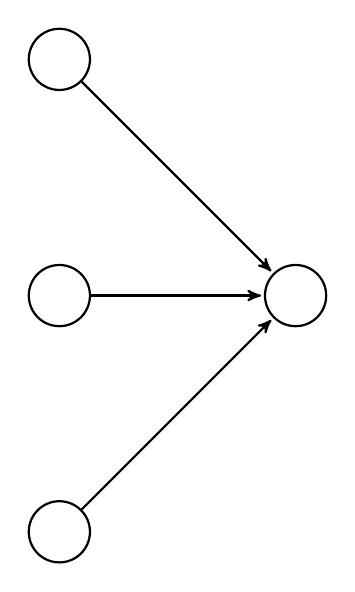
\begin{tikzpicture}[->,>=stealth',shorten >=1pt,auto,node distance=3cm,
  thick,main node/.style={circle,draw,font=\sffamily\Large\bfseries}]

  \node[main node] (0) {\phantom{0}};
  \node[main node] (2) [left  of=0] {\phantom{0}};
  \node[main node] (1) [above of=2] {\phantom{0}};
  \node[main node] (3) [below of=2] {\phantom{0}};

  \path[every node/.style={font=\sffamily\small}]
  (1) edge node [right] {} (0)
  (2) edge node [right] {} (0)
  (3) edge node [left] {} (0);
\end{tikzpicture}
\end{document}
